% !TEX root = report.tex

\section{Processing Pipeline}
\label{sec:processing_architecture}

High level descripion of the processing flow:

Throughout the report: extract Spectrograms, classify image.

\section{Signals and Features}
\label{sec:model}

\subsection{Google Dataset}

% Measurement setup, data preprocess (describe the google dataset)

The Speech Commands datasets, described in \cite{warden2018speech}, provides
thousands of one second recording of $35$ differen words. The recordings are
mainly of volounteers, who used their own device to record the words in a
closed room wherever they happened to be (not in a studio setting).
Ideally each volounteer only recorded the $135$ requested utterances once, so the
dataset provides good variability of voices.
The utterances have a duration of one second.
To more precisely align the recorded clips, the audio was acquired for $1.5$
seconds and the $1$ second clip that contained the highest overrall volume was
extracted.
Several background noise recording are included as well.
The full dataset includes $105829$ utterances of $35$ words, saved in
\textit{.wav} format at $16$ KHz rate.
The dataset is released under the Creative Commons BY $4.0$ License \cite{ccby4}.

The dataset ships with a function to split the data in train, validation and
test folds, as well as two example lists of validation data ($9981$ utterances)
and test data ($11005$ utterances).
Throughout the experiments, those lists were used.
% both for the practicality of having them ready, but also to keep with the
% spirit of the dataset as a tool to enable meaningf

\subsection{Mel spectrogram and Mel-frequency Cepstral Coefficients}

The audio data in the dataset is available as a vector of amplitudes over time,
sampled at $16$ KHz. In this representation, the classification task is quite
hard.
The Fourier transform allows to convert a signal from the time domain into the
frequency domain. The result is called spectrum of the signal. This transform
is efficiently computed using the Fast Fourier Transform algorithm.

The short-time Fourier transform accounts for variations of the content of an
audio signal over time. Instead of computing the FFT of the entire signal, the
FFT is computed on overlapping windowed segments of the signal: each window has
length \texttt{n_fft} and the next window is extracted after
\texttt{hop_length} samples.
The results of the FFT in each window are stacked to obtain the spectrogram.

The human ear does not perceive frequencies on a linear scale: the difference
between $200$ and $400$ Hz is very marked, whereas two notes at $8000$ and
$8200$ Hz are almost indistinguishable. The mel scale, proposed by Stevens,
Volkmann, and Newmann \cite{melscale1937}, introduces a unit of pitch built in
such a way that equal distances on the scale sound equally distant to the human
listener.
The mel spectrogram is a spectrogram where the frequencies are converted to the
mel scale. To do so, a Mel spaced filterbank is generated (a 10 filters version
is shown in \fig{fig:mel10_filterbank}) and the FFT results are multiplied with
a dot product with each filter, obtaining \texttt{n_mel} values for each
timestep.

\begin{figure}[t!]
    \centering
    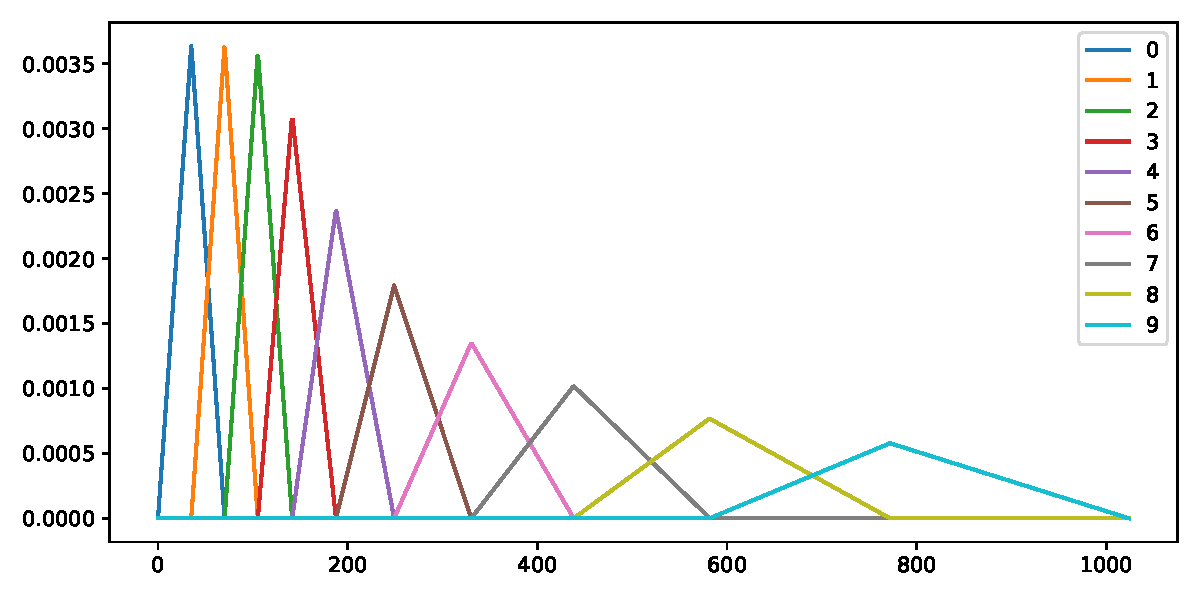
\includegraphics[width=0.8\linewidth]{mel10_filterbank.pdf}
    \caption{An example of a 10 filters Mel filterbank}
    \label{fig:mel10_filterbank}
\end{figure}

The resulting coefficients are highly correlated: the Discrete Cosine Transform
can be applied to decorrelate the filter bank coefficients and obtain a
compressed representation.
The results are the Mel-frequency Cepstral Coefficients.

An example waveform for the word ``happy'' and the relative spectrograms are
shown in \fig{fig:happy_specs}.

\begin{figure}[t!]
    \centering
    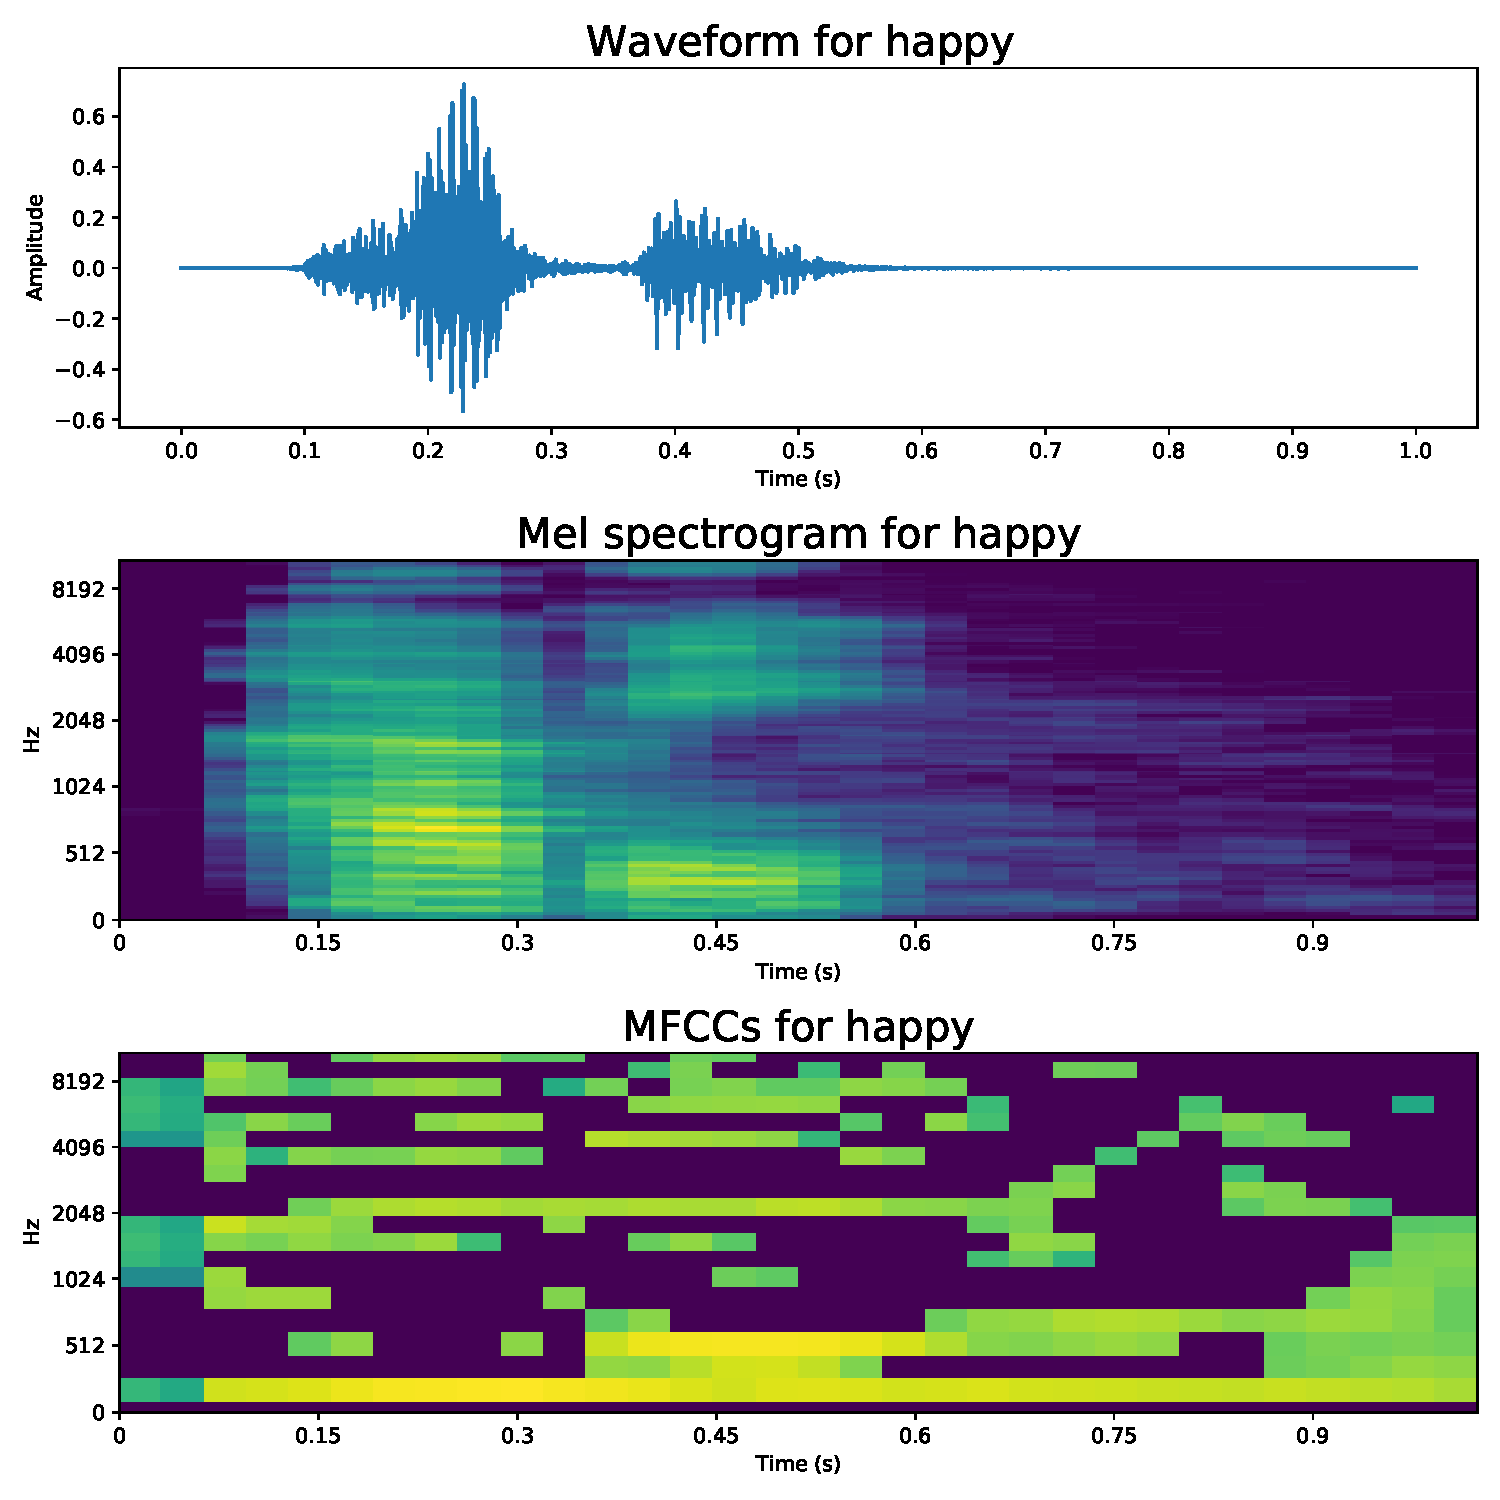
\includegraphics[width=0.8\linewidth]{happy_specs.pdf}
    \caption{Waveform and spectrograms for the word happy}%
    \label{fig:happy_specs}
\end{figure}

% The entire process is as follows:
% \begin{enumerate}
%     \item Split the signal in windows
%     \item Compute the FFT for each window
%     \item Convert to Mel scale
% \end{enumerate}

\subsection{Data augmentation}

\subsubsection{Time shift}

\subsubsection{Time stretch}

\subsubsection{Spectrogram warp}

\section{Learning Framework}
\label{sec:learning_framework}

How did it learn anything at all?

\subsection{Learning rate schedule}

\subsection{Hyper-parameter tuning}

\section{Convolutional Architecture}
\label{sec:convolutional_arch}

\section{Transfer Learning approach}
\label{sec:transfer_learning}

\section{Attention Model}
\label{sec:attention_model}

\subsection{Attention architecture}

\subsection{Query style}
